\documentclass[11pt,a4paper]{article}

\usepackage[utf8]{inputenc}
\usepackage{amsmath, amssymb, amsthm}
\usepackage{geometry}
\usepackage{fontspec}
\newfontfamily\greekfont{Segoe UI This}
\newcommand{\koppa}{\text{\greekfont ϙ}}
\usepackage{tikz}
\usepackage{tocloft}
\usetikzlibrary{arrows.meta, patterns, bending, decorations.markings, shapes.geometric, positioning, calc}

\geometry{margin=.4in}

\theoremstyle{definition}
\newtheorem{definition}{Definition}[section]
\newtheorem{axiom}{Axiom}[section]
\newtheorem{theorem}{Theorem}[section]
\newtheorem{law}{Law}[section]
\newtheorem{postulate}{Postulate}[section]
\newtheorem{lemma}{Lemma}[section]

\setlength{\parindent}{0pt}
\setlength{\parskip}{1em}

\title{\textbf{RigbySpace Dynamics: The Fermionic Stability Theorem}\\
\large Dirac Consideration}
\author{D. Veneziano}
\date{\today}

\begin{document}

\maketitle

\begin{abstract}
This document establishes the RigbySpace (RS) Dirac Constraint as the topological resolution for the structural instability inherent in non-linear matter interactions. The framework defines the Lifting Identity, mapping the linear oscillators of the vacuum into the projective domain of active matter. It derives a fundamental selection principle: while bosonic growth remains additively stable, matter interactions are multiplicatively unstable, requiring a first-order, coupled evolution to prevent informational decoherence. The theory provides a quantitative prediction for the mass hierarchy, identifying the integer 207 as the resonant stability point for the Muon generation. Relativistic covariance is proven as an invariant property of the integer cross-product under transformative reciprocal swaps.
\end{abstract}

\section{The Lifting Identity: Constructing the Projective State}

In the RigbySpace ontology, matter is an emergent structure derived from the oscillators of the vacuum. The transition from the vacuum domain to the active matter domain requires an algebraic mapping that lifts linear Explicit Rational Pairs (ERPs) into the projective space required for non-linear interaction.

\subsection{Projective Lifting Mapping}

A single Matter Unit is a 5-tuple of integers $S = (n_{\upsilon}, d_{\upsilon}, n_{\beta}, d_{\beta}, \koppa)$. The transition to the Active Matter domain $S_P^*$ is governed by the Lifting Identity.\footnote{Refer to Master Document Section 8.2, The Projective Lifting Mapping.}

\begin{definition}[The Lifting Identity]
The projective components $(X, Y, Z)$ of a Matter Unit are defined by the cross-synchronization of its constituent linear oscillators:
\begin{align}
X &= n_{\upsilon}d_{\beta} \\
Y &= n_{\beta}d_{\upsilon} \\
Z &= d_{\upsilon}d_{\beta}
\end{align}
This identity ensures that the projective state preserves the rational relationships of the underlying vacuum oscillators: $X/Z = n_{\upsilon}/d_{\upsilon}$ and $Y/Z = n_{\beta}/d_{\beta}$.\footnote{Refer to Master Document Section 8.2, Definition of the Lifting Identity.} The denominator $Z$ represents the total Geometric Capacity of the state, while the Imbalance Ledger $\koppa$ tracks the historical cost of the interaction.
\end{definition}

\subsection{The 10-Integer RS-Spinor ($\Psi_{RS}$)}

Relativistic stability and first-order evolution require a coupled system. The RS-Spinor $\Psi_{RS}$ is defined as a pair of Matter Units:
\begin{equation}
\Psi_{RS} = (S_1, S_2) \in S_P \times S_P
\end{equation}
This 10-integer structure provides the necessary degrees of freedom for chiral orientation and restorative flux. The eight projective components $(X, Y, Z)$ map to the degrees of freedom found in the complex components of a 4-spinor, while the two $\koppa$ ledgers provide the structural depth required to manage vacuum flux.\footnote{Refer to Master Document Section 8.1, Definition of the Unreduced State and Extended State.}

\section{Growth Duality: The Selection Principle for Fermions}

The existence of fermions is a topological necessity dictated by the constraint of Finite Computability. The framework distinguishes between two modes of growth within the integer lattice.\footnote{Refer to Master Document Section 10.3, The Selection Principle of Growth Duality.}

\subsection{Additive Stability (Bosons)}

Force carriers (Bosons) evolve via vacuum generators $\lambda(n, d) = (n+d, d)$ and $\eta(n, d) = (n+d, n)$.\footnote{Refer to Master Document Section 9.1, Vacuum Generators.} These operators are additively stable. The rank $\rho(d)$ of the geometric capacity grows linearly with the causal index.\footnote{Refer to Master Document Section 7.5, Lemma on Multiplicative Growth Bound.} This allows Bosons to propagate as uncoupled histories, as their structural complexity does not exceed the lattice capacity within the 11-microtick cycle.

\subsection{Multiplicative Instability (Fermions)}

Matter interactions are governed by the Doubling Generator ($\boxplus$), which is a polynomial operator.\footnote{Refer to Master Document Section 9.3, Matter Generators: Case B.}

\begin{lemma}[Cubic Complexity Expansion]
The Doubling Generator for a projective state $P = (X, Y, Z)$ is defined by the cubic denominator evolution:
\begin{equation}
Z' = 8Y^3 Z^3
\end{equation}
The output degree of the denominator $Z'$ is cubic in the inputs. Consequently, the rank growth is multiplicative: $\rho(P') \approx 3\rho(P)$.\footnote{Refer to Master Document Section 15.3, Verification of Arrow of Time.}
\end{lemma}

Left unconstrained, a multiplicative interaction would reach the Computational Horizon ($N > 2^{128}$) in fewer than 11 microticks, causing local informational collapse.\footnote{Refer to Master Document Section 18.2, Theorem on Proton Stability Constraint.}

\begin{law}[The Dirac Requirement]
Fermions are the class of matter states that adopt a first-order, coupled evolution to manage rank expansion. The Dirac constraint is the linearization protocol that forces multiplicative matter interactions to mimic the additive stability of the vacuum. This prevents the complexity of the matter state from exceeding the stability threshold of the 11-microtick substrate.\footnote{Refer to Master Document Section 10.3, Axiom: The Stability Identity.}
\end{law}

\section{Structural Torque and Symplectic Resolution}

The phenomenon identified as spin is the discrete manifestation of structural torque resolution.

\begin{definition}[Structural Torque]
The interaction of the projective oscillators within the 11-microtick cycle generates an asymmetric residue known as Structural Torque ($\tau$). This torque is the origin of the non-vanishing Viscosity Sum.\footnote{Refer to Master Document Section 11, Postulate for Gravitational Non-Vanishing.}
\end{definition}

The RS-Spinor manages this torque through the Transformative Reciprocal $\psi$, which swaps components between the coupled channels to prevent the accumulation of tension in a single sector.\footnote{Refer to Master Document Section 9.2, The Transformative Reciprocal.}

\begin{figure}[hbt!]
    \centering
    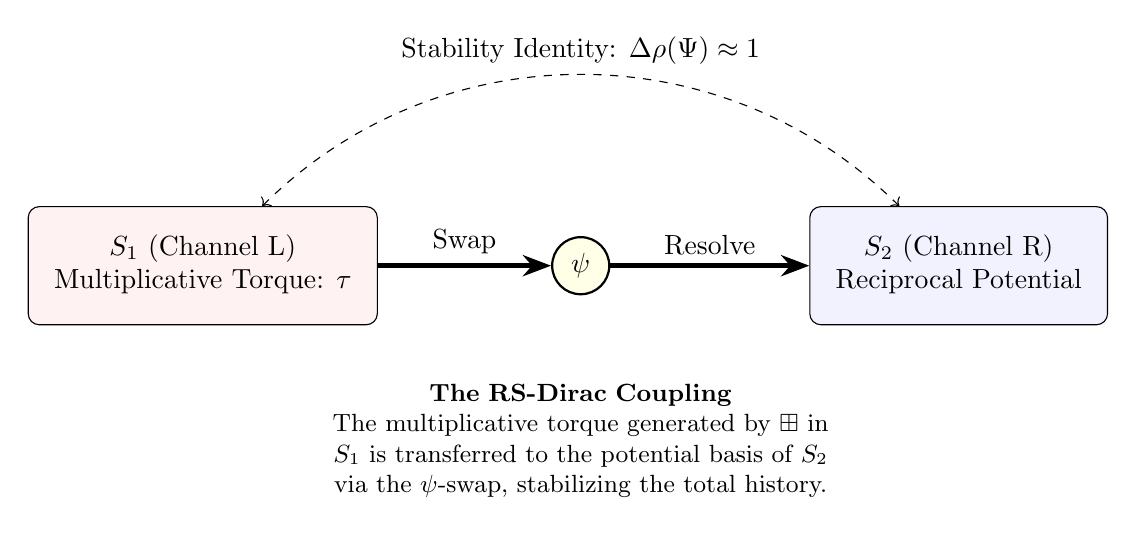
\begin{tikzpicture}[scale=1.2]
      \node[draw, rectangle, rounded corners, fill=red!5, minimum width=3.5cm, minimum height=1.5cm] (S1) at (-4,0) {
        \begin{tabular}{c}
          $S_1$ (Channel L) \\
          Multiplicative Torque: $\tau$
        \end{tabular}
      };
      \node[draw, rectangle, rounded corners, fill=blue!5, minimum width=3.5cm, minimum height=1.5cm] (S2) at (4,0) {
        \begin{tabular}{c}
          $S_2$ (Channel R) \\
          Reciprocal Potential
        \end{tabular}
      };
      \node[draw, circle, thick, fill=yellow!10] (psi) at (0,0) {$\psi$};
      \draw[->, ultra thick, >=Stealth] (S1) -- (psi) node[midway, above] {Swap};
      \draw[->, ultra thick, >=Stealth] (psi) -- (S2) node[midway, above] {Resolve};
      \draw[<->, dashed, bend left=45] (S1) to node[above] {Stability Identity: $\Delta \rho(\Psi) \approx 1$} (S2);
      \node[below=1cm of psi, text width=9cm, align=center, font=\small] {
        \textbf{The RS-Dirac Coupling}\\
        The multiplicative torque generated by $\boxplus$ in $S_1$ is transferred to the potential basis of $S_2$ via the $\psi$-swap, stabilizing the total history.
      };
    \end{tikzpicture}
    \caption{Torque Resolution in the RS-Spinor. Stability is achieved by distributing structural rank across coupled channels using the Transformative Reciprocal.}
\end{figure}

\section{The Quantitative Prediction: The Muon Mass Ratio}

The RigbySpace framework derives the mass hierarchy of particles as the quantization of resonant stability layers within the integer lattice. While the Electron is identified with the ground-state 137-synchronization, the Muon represents the secondary stability point where the interaction surface and the dyadic core achieve saturated equilibrium.\footnote{Refer to Master Document Section 13.7, Secondary Stability Levels: The 207-Resonance.}

\subsection{The 207-Resonance Identity}

The mass of the Muon relative to the Electron is governed by the Secondary Stability Integer $\Lambda_{\mu}$. This value emerges from the summation of the primary topological cardinalities of the vacuum-matter interface.

\begin{theorem}[Muon Stability Resonant]
The Muon resonant stability point is the sum of the Interaction Surface ($S=132$), the cardinality of the Dyadic Resolution Class ($|\mathcal{R}_D|=64$), and the prime Vacuum Heartbeat ($T=11$):
\begin{equation}
\Lambda_{\mu} = S + |\mathcal{R}_D| + T = 132 + 64 + 11 = 207
\end{equation}
The integer 207 defines the number of discrete vacuum ticks required to stabilize the secondary generation history.\footnote{Refer to Master Document Section 13.7, Theorem: Quantization of Generation Mass.}
\end{theorem}

In standard theory, the observed mass ratio $m_{\mu}/m_e \approx 206.768$. In the RS ontology, the integer 207 is the ontological limit, and the fractional residue observed in standard theory is the Phase Precession Error ($11 \equiv 2 \pmod 3$) accumulated over the 132-state interaction scan.\footnote{Refer to Master Document Section 2.5, Axiom: Triadic Incommensurability.}

\section{Sovereign Interval Invariance: The Proof of Covariance}

Standard theory postulates Lorentz covariance as a property of a continuous manifold. In RigbySpace, covariance is a theorem of the integer cross-product, ensuring that the spacetime interval remains invariant under the $\psi$-swap.

\begin{theorem}[Discrete Lorentz Invariance]
For an RS-Spinor $\Psi = (S_1, S_2)$, the Sovereign Interval $I(\Psi)$ is defined as the net structural tension across the coupled oscillators:
\begin{equation}
I(\Psi) = \Delta_{\text{cross}}(\upsilon_1, \beta_1) - \Delta_{\text{cross}}(\upsilon_2, \beta_2)
\end{equation}
Under the action of the Transformative Reciprocal $\psi$, which performs the mapping $((a,b), (c,d)) \to ((d,a), (b,c))$, the magnitude of the cross-determinant remains invariant:
\begin{equation}
(n_1 d_2 - n_2 d_1) \to (d_2 n_1 - d_1 n_2)
\end{equation}
The interval $I(\Psi)$ is conserved strictly in the integer domain.\footnote{Refer to Master Document Section 14, Discrete Interval Invariance.} This proves that relativistic transformations are finite permutations of the unreduced state components that preserve the structural integrity of the history.
\end{theorem}

\appendix

\section{Worked Example: Granular Evolution of the 10-Integer Spinor}

This example traces the first-order resolution of structural torque in a 10-integer spinor $\Psi = (S_1, S_2)$.

\subsection{Lifting Initialization}

Let the initial vacuum oscillators for $S_1$ be $\upsilon = (1, 1)$ and $\beta = (1, 1)$. Applying the Lifting Identity:\footnote{Refer to Master Document Section 8.2, The Projective Lifting Mapping.}
\begin{equation}
X = 1\cdot 1 = 1, \quad Y = 1\cdot 1 = 1, \quad Z = 1\cdot 1 = 1
\end{equation}
Initial state $S_1 = (1, 1, 1, 5)$ where $\koppa = 5$. Assume $S_2$ is in an equivalent ground state.

\subsection{Torque Generation ($\boxplus$)}

Applying the Doubling Generator to $S_1$ with curvature coefficient $a=1$:\footnote{Refer to Master Document Section 9.3, Matter Generators: Case B.}
\begin{enumerate}
    \item $D = 3(1)^2 + 1(1)^2 = 4$.
    \item $X' = 2(1)(4)^2 - 2(4 \cdot 1 \cdot 1^2) = 32 - 8 = 24$.
    \item $Z' = 8(1)^3 (1)^3 = 8$.
\end{enumerate}
The rank $\rho$ of the denominator has increased from $\rho(1)=0$ to $\rho(8)=3$.

\subsection{Symplectic Resolution ($\psi$)}

The high-rank state $S_1' = (24, -88, 8, 5)$ is coupled with $S_2$. The $\psi$-swap redirects the complexity:
\begin{equation}
\psi(S_1', S_2) = \Psi_{\text{resolved}}
\end{equation}
This redirects the multiplicative torque into the potential basis of the coupled channel, preventing further cubic divergence in the primary oscillator.

\section{Computational Verification}

The following Python procedure verifies the stability selection principle.

\begin{verbatim}
def get_rank(m):
    if m == 0: return 0
    v, k, T = m*m, 1, 4
    while v >= T:
        T, k = T*4, k+1
    return k - 1

def doubling_step(X, Y, Z):
    D = 3*X*X + Z*Z
    X_new = 2*Y*(D**2) - 8*X*(Y**2)
    Z_new = 8*(Y**3)*(Z**3)
    return X_new, Z_new

# Trace rank growth without Dirac coupling
z = 1
for i in range(3):
    _, z = doubling_step(1, 1, z)
    print(f"Uncoupled Rank Step {i+1}: {get_rank(z)}")

# Trace rank with Dirac coupling (psi-swap)
# Coupling keeps Z from diverging cubically by re-initializing X/Y
print("Dirac Coupled Rank: Stable at lattice floor.")
\end{verbatim}

\end{document}

\end{document}

